% ==============================================================================
%
%                             Communication
%
% ==============================================================================
\chapter{Communication} \label{chapt:comm}
In the following chapter the communication part of the project is
explained. A rough introduction to the VHDL design flow shows how the code is
written. Then the requirements are stated and a system overview is shown in
chapter \ref{chapt:comm:concept}. A custom session protocol is defined on top of
UDP and then implemented using VHDL.

% ==============================================================================
%
%                             Vivado Design Flow
%
% ==============================================================================
\section{Design Flow}
Figure \ref{fig:vhdldesignflow} shows the standard design flow applied on
projects using hardware description language (HDL). In this project VHDL is
used as the main language. The first step in a design is the system analysis.
The requirements are broken down into blocks. Their relations are recorded in
a block design. Then the VHDL code is written per block alongside of a testbench
that tests the functionality of the block. The simulation reads these two files,
stimulates the block and verifies the output. If all requirements are met, the
synthesis and implementation is run. It converts the hardware description
language to a netlist on gate level. Timing simulations are run by the synthesis
tool. If not all timing requirements are met the synthesis can be run using
different parameters or the VHDL code must be altered. The final test is running
the code on the FPGA and testing the results.

\begin{figure}[tb!]
    \centering
    \begin{tikzpicture}[
    rounded corners=0mm,
]
    %coordinates
    \coordinate (analysis)      at (0,-1);
    \coordinate (bd) at (0,-2);
    \coordinate (wrvhdl)      at (-3,-5);
    \coordinate (wrtb)      at (3,-5);
    \coordinate (sim)      at (0,-6.5);
    \coordinate (synimpl)      at (0,-8);
    \coordinate (timing)     at (0,-9.5);
    \coordinate (onfpga)     at (0,-10.5);

    %nodes
    \node[draw, minimum width=4cm, anchor=south, text width=3.8cm, align=center] (n1) at (analysis) {System Analysis};
    \node[draw, minimum width=4cm, anchor=south, text width=3.8cm, align=center] (n2) at (bd) {Block Design};
    \node[draw, minimum width=4cm, minimum height=1.5cm,  anchor=south, text width=3.8cm, align=center] (n3) at (wrvhdl) {Write VHDL Code per Block};
    \node[draw, minimum width=4cm, minimum height=1.5cm,  anchor=south, text width=3.8cm, align=center] (n4) at (wrtb) {Write VHDL Testbench};
    \node[draw, minimum width=4cm, anchor=south, text width=3.8cm, align=center] (n5) at (sim) {Simulate};
    \node[draw, minimum width=4cm, anchor=south, text width=3.8cm, align=center] (n6) at (synimpl) {Synthesis and Implementation};
    \node[draw, minimum width=4cm, anchor=south, text width=3.8cm, align=center] (n7) at (timing) {Check timing Requirements};
    \node[draw, minimum width=4cm, anchor=south, text width=3.8cm, align=center] (n8) at (onfpga) {On FPGA test};
    
    \path[draw,-{Latex[length=2.5mm]}] (n1) -- (n2) ;
    \path[draw,-{Latex[length=2.5mm]}] (n5) -- (n6) ;
    \path[draw,-{Latex[length=2.5mm]}] (n6) -- (n7) ;
    \path[draw,-{Latex[length=2.5mm]}] (n7) -- (n8) ;

    \path[draw,-{Latex[length=2.5mm]}] (n2) -- ($(n2) + (0,-1)$) -| (n4) ;
    \path[draw,-{Latex[length=2.5mm]}] (n2) -- ($(n2) + (0,-1)$) -| (n3) ;

    \path[draw,-{Latex[length=2.5mm]}] (n4) |- (n5) ;
    \path[draw,-{Latex[length=2.5mm]}] (n3) |- (n5) ;
    \path[draw,-{Latex[length=2.5mm]}] (n5) |- (n3) ;
    \path[draw,-{Latex[length=2.5mm]}] (n5) |- (n4) ;

    \path[draw,-{Latex[length=2.5mm]}] (n7) -- ($(n7) + (-3,0)$) |- (n6) ;

    \path[draw,-{Latex[length=2.5mm]}] (n8) -- ($(n8) + (-6,0)$) |- (n3) ;
    \path[draw,-{Latex[length=2.5mm]}] (n8) -- ($(n8) +  (6,0)$) |- (n4) ;

\end{tikzpicture}
    \caption{VHDL Design Flow}
    \label{fig:vhdldesignflow}
\end{figure}

% ==============================================================================
%
%                             Requirements
%
% ==============================================================================
\section{Requirements}
As mentioned at the end of chapter \ref{chapt:mission:possible:communication} the session
layer has to be implemented in hardware. The requirements are as followed:
\\

\textbf{Speed:}
The main goal of the project is to have fast image processing.
Therefore the communication must not be a bottleneck. The AC701
Evaluation Kit features a Gigabit Ethernet PHY \cite{xilinx_ac701}. The
communication therefore has to meet the speed requirements of 125MB/s
\footnote{Considering the overhead of the underlaying protocols, the
throughput may be a bit less than 125MB/s} \cite{8023}.
\\

\textbf{Communication overhead:}
To maximize the throughput on the Gigabit Ethernet channel the data overhead
must be minimal. 
\\

\textbf{Scalability:}
The communication must work on a network with multiple FPGAs.
\\

\textbf{Implementation effort:}
The communication protocol is implemented directly in FPGA hardware where area
is limited. The smaller the communication implementation is, the more area is
left for the image processing algorithm.

\textbf{Underlaying protocol:}
For the communication to work on a local area network (LAN), underlaying protocols
have to be applied. The layer 3 (IPv4) and layer 4 (UDP) are handled by the UDP IP
Stack IP Core from Opencores \cite{udpipstack} therefore the communication has
to be based on UDP.
\\

\textbf{Data loss:}
Since UDP is used as layer 4 protocol, reliable data transmission is not
guaranteed. To ensure that all image data is transmitted to the FPGA the
communication protocol must implement an acknowledge functionality to enable data
retransmission.

% ==============================================================================
%
%                             Concept
%
% ==============================================================================
\section{Concept} \label{chapt:comm:concept}
To meet all requirements, a custom layer 5 protocol is implemented, UDP File
Transfer or UFT for short. It communicates with the UDP IP Stack which in turn
connects to the Xilinx Tri-Mode Ethernet Medium Access Controller. Figure 
\ref{fig:commoverview} shows the top level block design. The UDP File Transfer
block is implemented from scratch. It implements the UDP File Transfer protocol
defined in section \ref{chapt:protospec}. The UFT block communicates to the
UDP Stack using AXI stream interfaces for tx and rx data and control signals
containing UDP and IP header information, start and stop bits.

\vspace{2em}
\begin{figure}[h!]
    \centering
    % \tikzsetnextfilename{system-overview}
\begin{tikzpicture}[
    rounded corners=0mm,
]
    %coordinates
    \coordinate (orig)      at (0,0);
    \coordinate (c1)        at (2.5,0);
    \coordinate (c2)        at (6,0);
    \coordinate (c3)        at (0,0);
    \coordinate (c4)        at (0,0);



    \coordinate (otemacsup) at (4,0);
    \coordinate (ophy)      at (0,-2);
    \coordinate (omac)      at (0,0);
    \coordinate (oudp)      at (8,0);
    \coordinate (ouft)      at (12,0);
    \coordinate (oamb1)     at (16,1);
    \coordinate (oamb2)     at (16,3);

    %nodes

    \begin{pgfonlayer}{main}
        \node[draw, fill=white, minimum width=2cm, minimum height=3cm, anchor=west, text width=2cm, align=center] (mac) at (c1) {Xilinx Tri-Mode Ethernet MAC};
        \begin{scope}[yshift=0cm,node distance=1.5cm]
            \node[draw, fill=white, right = of mac, minimum width=2cm, minimum height=3cm, anchor=west, text width=2cm, align=center] (udp) {Opencores UDP IP Stack};
            \node[draw, fill=white, right = of udp, minimum width=2cm, minimum height=3cm, anchor=west, text width=2cm, align=center] (uft) {UDP File Transfer};
        \end{scope}
        \node[right = 0.8cm of uft, minimum width=2cm, minimum height=1cm, anchor=west, text width=2cm, align=center] (axi) {AXI Memory Mapped};

        \node[draw, below = 1.8cm of mac, fill=white, minimum width=2cm, minimum height=1cm, anchor=south, text width=1cm, align=center] (phy) {PHY};
        \node[fill=white, left = 3.0cm of phy, minimum width=1.5cm, minimum height=1cm, anchor=west, text width=1.5cm, align=center] (eth) {Gigabit Ethernet};
    \end{pgfonlayer}

    % FPGA box
    \begin{pgfonlayer}{main}
        \node[] (FPGA) at ($(mac) + (-1.0,2.0)$) { FPGA };
    \end{pgfonlayer}
    \begin{pgfonlayer}{foreground}
        \node (f_fpga) [draw=black, fill=gray!20, inner sep=5, fit={(FPGA) (mac) (udp) (uft) (axi)}] {};
    \end{pgfonlayer} 

    % Board box
    \begin{pgfonlayer}{main}
        \node[] (board) at ($(mac) + (-0.0,3.0)$) { AC701 Evaluation Kit };
    \end{pgfonlayer}
    \begin{pgfonlayer}{background}
        \node (f_board) [draw=black, fill=gray!40, inner sep=5, fit={(board) (f_fpga) (phy)}] {};
    \end{pgfonlayer} 

    
    \path[draw,{Latex[length=2.5mm]}-{Latex[length=2.5mm]}] (eth) -- (phy) ;
    \path[draw,{Latex[length=2.5mm]}-{Latex[length=2.5mm]}] (phy) -- (mac) node [midway, label=right:RGMII] {};
    \path[draw,{Latex[length=2.5mm]}-{Latex[length=2.5mm]}] (mac) -- (udp) node [midway, label=above:AXI\_S] {};
    \path[draw,{Latex[length=2.5mm]}-{Latex[length=2.5mm]}] ($(udp.0) + (0,1.5/2)$) -- ($(uft.180) + (0,1.5/2)$) node [midway, label=above:AXI\_S] {};
    \path[draw,{Latex[length=2.5mm]}-{Latex[length=2.5mm]}] (udp) -- (uft) node [midway, label=above:control] {};
    \path[draw,{Latex[length=2.5mm]}-{Latex[length=2.5mm]}] ($(udp.0) + (0,-1.5/2)$) -- ($(uft.180) + (0,-1.5/2)$) node [midway, label=above:hdr] {};
    \path[draw,{Latex[length=2.5mm]}-{Latex[length=2.5mm]}] (uft) -- (axi) ;

    % \path[draw,{Latex[length=2.5mm]}-{Latex[length=2.5mm]}] (B) |- ($(B)!1/2!(B |- D)$) coordinate (xx) -| ($(D.270) + (0,0)$);
    % \path[draw,{Latex[length=2.5mm]}-{Latex[length=2.5mm]}] (C) |- ($(C)!1/2!(C |- D)$) coordinate (xx) -| ($(D.270) + (1/2,0)$);
  
\end{tikzpicture}
    \caption{Communication Overview}
    \label{fig:commoverview}
\end{figure}
\clearpage

% ==============================================================================
%
%                             Protocol Specification
%
% ==============================================================================
\section{Protocol Specification} \label{chapt:protospec}
The goal of the UDP File Transfer protocol (UFT) is to transmit files using
the UDP protocol. UDP lacks data segmentation and reliable transfer. These
features are implemented in UFT. Detailed protocol specifications are attached
in appendix \ref{app:uftspec}.\\

UFT sends either a data or a control packet (see table \ref{tab:uftcommand} and \ref{tab:uftdata}). The first bit determines the packet
type. The control packet contains a command and two command data fields. Table \ref{tab:uftcommandlist} shows a list of
all commands. The
data packet consists of the transaction ID (TCID), packet sequence number 
(SEQNBR) and the data.

The transaction ID (TCID) uniquely identifies each data packet to a running file
transmission. The TCID is incremented after a successful transmission. If a file
exceeds the maximum packet size of 1464 Bytes it is fragmented into sequences.
The sequence number (SEQNBR) enumerates these fragments so the receiver can
reassemble the file accordingly.

A file transmission is initiated with a file transfer start (FTS) command. The
packet tells the receiver the new transaction ID and how many sequences are
going to be transmitted (NSEQ). The sender then begins to send the data packets
with the according TCID and SEQNBR. The receiver acknowledges every
data packet received with a acknowledge data packet command (ACKFP). If all packets are
received, the receiver sends a acknowledge file transfer (ACKFT) command. A
transmission can always be aborted by sending a file transfer stop (FTP) command
by either the sender or the receiver.

\begin{table}[]
\centering
\begin{adjustbox}{max width=\textwidth}
\begin{tabular}{l|llllllll|llllllll|llllllll|llllllll|}
 & 0 &  &  &  &  &  &  &  & 1 &  &  &  &  &  &  &  & 2 &  &  &  &  &  &  &  & 3 &  &  &  &  &  &  &  \\
 & \multicolumn{1}{l|}{0} & \multicolumn{1}{l|}{1} & \multicolumn{1}{l|}{2} & \multicolumn{1}{l|}{3} & \multicolumn{1}{l|}{4} & \multicolumn{1}{l|}{5} & \multicolumn{1}{l|}{6} & 7 & \multicolumn{1}{l|}{0} & \multicolumn{1}{l|}{1} & \multicolumn{1}{l|}{2} & \multicolumn{1}{l|}{3} & \multicolumn{1}{l|}{4} & \multicolumn{1}{l|}{5} & \multicolumn{1}{l|}{6} & 7 & \multicolumn{1}{l|}{0} & \multicolumn{1}{l|}{1} & \multicolumn{1}{l|}{2} & \multicolumn{1}{l|}{3} & \multicolumn{1}{l|}{4} & \multicolumn{1}{l|}{5} & \multicolumn{1}{l|}{6} & 7 & \multicolumn{1}{l|}{0} & \multicolumn{1}{l|}{1} & \multicolumn{1}{l|}{2} & \multicolumn{1}{l|}{3} & \multicolumn{1}{l|}{4} & \multicolumn{1}{l|}{5} & \multicolumn{1}{l|}{6} & 7 \\ \hline
0 & \multicolumn{1}{l|}{0} & \multicolumn{7}{l|}{Command {[}6:0{]}} & \multicolumn{24}{l|}{Command Data 1 {[}23:0{]}} \\ \hline
4 & \multicolumn{32}{l|}{Command Data 2 {[}31:0{]}} \\ \hline
8 & \multicolumn{32}{l|}{Padding 26 Bytes} \\ \hline
\end{tabular}
\end{adjustbox}
\caption{UFT Command Packet}
\label{tab:uftcommand}
\end{table}

\begin{table}[]
\centering
\begin{adjustbox}{max width=\textwidth}
\begin{tabular}{l|llllllll|llllllll|llllllll|llllllll}
 & 0 &  &  &  &  &  &  &  & 1 &  &  &  &  &  &  &  & 2 &  &  &  &  &  &  &  & 3 &  &  &  &  &  &  &  \\
 & \multicolumn{1}{l|}{0} & \multicolumn{1}{l|}{1} & \multicolumn{1}{l|}{2} & \multicolumn{1}{l|}{3} & \multicolumn{1}{l|}{4} & \multicolumn{1}{l|}{5} & \multicolumn{1}{l|}{6} & 7 & \multicolumn{1}{l|}{0} & \multicolumn{1}{l|}{1} & \multicolumn{1}{l|}{2} & \multicolumn{1}{l|}{3} & \multicolumn{1}{l|}{4} & \multicolumn{1}{l|}{5} & \multicolumn{1}{l|}{6} & 7 & \multicolumn{1}{l|}{0} & \multicolumn{1}{l|}{1} & \multicolumn{1}{l|}{2} & \multicolumn{1}{l|}{3} & \multicolumn{1}{l|}{4} & \multicolumn{1}{l|}{5} & \multicolumn{1}{l|}{6} & 7 & \multicolumn{1}{l|}{0} & \multicolumn{1}{l|}{1} & \multicolumn{1}{l|}{2} & \multicolumn{1}{l|}{3} & \multicolumn{1}{l|}{4} & \multicolumn{1}{l|}{5} & \multicolumn{1}{l|}{6} & 7 \\ \hline
0 & \multicolumn{1}{l|}{1} & \multicolumn{7}{l|}{Transaction ID {[}6:0{]}} & \multicolumn{24}{l|}{Packet sequence number {[}23:0{]}} \\ \hline
4 & \multicolumn{32}{l|}{Data} \\ \hline
\end{tabular}
\end{adjustbox}
\caption{UFT Data Packet}
\label{tab:uftdata}
\end{table}


\begin{table}[b!]
    \centering
    \begin{tabular}{l l l l l}
        \toprule
        Command & Short & Name & Data 1 & Data 2 \\
        \midrule
        0x00 & FTS & 
        File transfer start & TCID & NSEQ
        \\
        0x01 & FTP &
        File transfer stop & TCID & 0x0000 0000
        \\
        0x02 & ACKFP &
        Acknowledge data packet & TCID & SEQNBR
        \\
        0x03 & ACKFT &
        Acknowledge file transfer & TCID & 0x0000 0000
        \\
        \bottomrule
    \end{tabular}
    \caption{UFT command list}
    \label{tab:uftcommandlist}
\end{table}

% ==============================================================================
%
%                             Used Cores
%
% ==============================================================================
% \section{Used Cores}
% Der Tri Mode Ethernet MAC und der UDP IP Stack wird verwendet. Ein- und Ausgange 
% beschreiben und wie sie verwendet werden sollen.

% ==============================================================================
%
%                             UDP File Transfer Stack
%
% ==============================================================================
\section{UDP File Transfer Stack}

\begin{figure}[tb!]
    \centering
    \begin{adjustbox}{max width=\textwidth}
        % \tikzsetnextfilename{system-overview}
\begin{tikzpicture}[
    rounded corners=0mm,
    entity/.style={
        draw,
        minimum height=1.0cm,
        minimum width=3cm,
        fill=white,
        anchor=north west,
    },
]
    %coordinates
    \coordinate (orig)      at (0,0);
    \coordinate (crx)       at (0,0);
    \coordinate (crxmem)    at (5,0);
    \coordinate (crxamb)    at (10,0);

    \coordinate (ctxctl)    at (0,-2.5);
    \coordinate (ctxcmd)    at (5,-3.5);
    \coordinate (ctxdat)    at (5,-5.5);
    \coordinate (ctxamb)    at (0,-5.5);
    \coordinate (ctxarb)    at (10,-4.5);

    %nodes

    \begin{pgfonlayer}{main}
        % entities
        \node[entity, label={uft\_rx}] (rx) at (crx) {};
        \node[entity, label={[name=rxl] uft\_rx\_mem\_ctl}] (rxmem) at (crxmem) {};

        \node[entity, label={[name=ltxctl] uft\_tx\_ctl}] (txctl) at (ctxctl) {};
        \node[entity, label={[name=txcal]uft\_tx\_cmd\_assembler}] (txcmd) at (ctxcmd) {};
        \node[entity, label={uft\_tx\_data\_assembler}] (txdat) at (ctxdat) {};
        \node[entity, label={uft\_tx\_arbiter}] (txarb) at (ctxarb) {};

        \node[entity, label={axi\_master\_burst}] (ambrx) at (crxamb) {};
        \node[entity, label={axi\_master\_burst}] (ambtx) at (ctxamb) {};

        % ports
        \path[draw,{Latex[length=2.5mm]}-] ($(rx.180) + (0,1/6)$) -- ($(rx.180) + (-1.0,1/6)$) node[anchor=east] {rx\_hdr};
        \path[draw,{Latex[length=2.5mm]}-] ($(rx.180) + (0,-1/6)$) -- ($(rx.180) + (-1.0,-1/6)$) node[anchor=east] {s\_axi};
        \path[draw,{Latex[length=2.5mm]}-] ($(txctl.180) + (0,0)$) -- ($(txctl.180) + (-1.0,0)$) node[anchor=east] {controll};
        \path[draw,{Latex[length=2.5mm]}-] ($(ambtx.180) + (0,0/6)$) -- ($(ambtx.180) + (-1,0/6)$) node[anchor=east] {AXI};

        \path[draw,-{Latex[length=2.5mm]}] ($(ambrx.0) + (0,0)$) -- ($(ambrx.0) + (1.5,0/6)$) node[anchor=west] {AXI};
        \path[draw,-{Latex[length=2.5mm]}] ($(txctl.0) + (0,3.5/10)$) -- ($(txctl.0) + (11.5,3.5/10)$) node[anchor=west] {tx\_hdr};
        \path[draw,-{Latex[length=2.5mm]}] ($(txarb.0) + (0,0/10)$) -- ($(txarb.0) + (1.5,0/10)$) node[anchor=west] {s\_axi};

        % Interconnects
        \path[draw,-{Latex[length=2.5mm]}] ($(rx.0) + (0,1/6)$) -- ($(rxmem.180) + (0,1/6)$) node[anchor=east] {};
        \path[draw,-{Latex[length=2.5mm]}] ($(rx.0) + (0,-1/6)$) -- ($(rxmem.180) + (0,-1/6)$) node[midway, anchor=north] {s\_axi};
        % \node at ($(rx.180) + (-0.5,-1/6)$) [circle,fill,inner sep=1.5pt]{};

        \path[draw,-{Latex[length=2.5mm]}] ($(txctl.0) + (0,1.5/10)$) -| ($(txcmd.180) + (-0.5,0)$) -- ($(txcmd.180) + (0,0)$) node[anchor=west] {};
        \path[draw,-{Latex[length=2.5mm]}] ($(txctl.0) + (0,-1.5/10)$) -| ($(txarb.180) + (-6,0)$) -- ($(txarb.180) + (0,0)$) node[anchor=west] {};
        \path[draw,-{Latex[length=2.5mm]}] ($(txctl.0) + (0,-3.5/10)$) -| ($(txdat.180) + (-1.5,1/6)$) -- ($(txdat.180) + (0,1/6)$) node[anchor=west] {};

        \path[draw,-{Latex[length=2.5mm]}] ($(txcmd.0) + (0,0)$) -| node[anchor=south] {s\_axi} ($(txarb.180) + (-0.5,1/4)$)  -- ($(txarb.180) + (0,1/4)$);
        \path[draw,-{Latex[length=2.5mm]}] ($(txdat.0) + (0,0)$) -| node[anchor=north] {s\_axi}($(txarb.180) + (-0.5,-1/4)$) -- ($(txarb.180) + (0,-1/4)$);

        \path[draw,-{Latex[length=2.5mm]}] ($(ambtx.0) + (0,-1/6)$) -- ($(txdat.180) + (0,-1/6)$) node[anchor=east] {};
        \path[draw,-{Latex[length=2.5mm]}] ($(rxmem.0) + (0,0/6)$) -- ($(ambrx.180) + (0,0)$) node[anchor=east] {};

        % Ack
        \path[draw=red,line width=0.5mm,-{Latex[length=2.5mm]}] ($(crxmem.0) + (1.5,-1)$) |- ($(crxmem.0) + (-1,-2)$) -| ($(ctxctl.0) + (2.5,0)$) node[midway, anchor=east] {};


    \end{pgfonlayer}

    % tx box
    \begin{pgfonlayer}{foreground}
        \node [draw, fill=gray!20, inner sep=10, fit={(ltxctl) (txctl) (txcmd) (txdat) (txarb) (txcal)}, label={[label distance=0.0cm]150:uft\_tx\_top}] (tx) {};
    \end{pgfonlayer} 

    % Board box
    \begin{pgfonlayer}{background}
        \node [draw, fill=gray!40, inner sep=10, fit={(tx) (rx) (rxmem) (rxl)}, label=uft\_top] (tx) {};
    \end{pgfonlayer} 

\end{tikzpicture}
    \end{adjustbox}
    \caption{UFT Top Block Design}
    \label{fig:ufttop}
\end{figure}

Figure \ref{fig:ufttop} shows the block design of the UDP file transfer
implementation \footnote{The two axi\_master\_burst are drawn inside the block
for convenience. Currently they are implemented outside the UFT block}. The
stack is split into a receiver path and a transmitter path. Both can be operated
independently. In the following chapters these two paths are explained in more
detail.

% ==============================================================================
%
%                             Receiver
%
% ==============================================================================
\subsection{Receiver} \label{chapt:uftreceiver}
The receiving path is split into two entities. The entity \texttt{uft\_rx}
analyzes the UFT header and outputs the following information:

\begin{table}[h!]
    \centering
    \begin{tabular}{l l}
        \toprule
        Signal & Description \\
        \midrule
        \texttt{is\_command}         & Set when the packet is a command packet\\
        \texttt{command\_code}       & The packet command code\\
        \texttt{command\_data1}      & The packet command data field 1\\
        \texttt{command\_data2}      & The packet command data field 2\\
        \texttt{command\_data\_valid} & Set when the previous 4 signals are valid\\
        % \midrule
        \texttt{is\_data}            & Set when the packet is a data packet\\
        \texttt{data\_tcid}          & Transaction ID of the data packet\\
        \texttt{data\_seq}           & Sequence number of the data packet\\
        \texttt{data\_meta\_valid}    & Set when the previous 3 signals are valid\\
        \bottomrule
    \end{tabular}
    \caption{\texttt{uft\_rx} output signals}
    \label{tab:uftrxsig}
\end{table}

The entity \texttt{uft\_rx\_mem\_ctl} then buffers the input data inside a FiFo (First
in First out) and stores it in memory after a packet has been received through its AXI
Memory Mapped interface. The FiFo is necessary because the AXI Stream signal
coming from the UDP IP Stack is 8 bits wide and the AXI Memory Mapped interface
has a bus width of 32 bits. This bus width conversion is realized by the entity
\texttt{fifo\_8i\_32o}. A block diagram of the entity is shown in figure \ref{fig:8to32fifo}. 
FiFo 1 through 4 are 8 bits wide. The 8 bit input is 
connected to each FiFo data input. The write enable bits are connected to a
shift register that circularly shifts one set bit so that the input data is
evenly distributed on the four FiFos. The outputs are tied together to a 32 bit
bus. Data can be written to the FiFo if the full bit is cleared. Data can be
read if the empty bit is cleared. This does not mean that all output bits are
valid, the user has to count the number of bytes stored to read valid data at
the output.
\\
\begin{figure}[tb!]
    \centering
    \begin{adjustbox}{max width=\textwidth}
        % \tikzsetnextfilename{system-overview}
\def\tikzbfifo#1#2{
    \begin{scope}[shift={#1}]
        \draw [fill=white](0,0) -- (4,0) -- (4,-2) -- (0,-2) -- (0,0);
        
        \node (name) at (2,-0.8) {FIFO};
        \node (name) at (2,-1.2) {#2};
        
        \node [anchor=west] (wren)    at (0,-1/2) {wr\_en};
        \node [anchor=west] (di)      at (0,-2/2) {data\_i};
        \node [anchor=west] (full)    at (0,-3/2) {full};

        \node [anchor=east] (wren)    at (4,-1/2) {rd\_en};
        \node [anchor=east] (di)      at (4,-2/2) {data\_o};
        \node [anchor=east] (full)    at (4,-3/2) {empty};
    \end{scope}
}
\def\tikzband#1{
    \begin{scope}[shift={#1}]
        \draw [fill=white](0,0) -- (1,0) -- (1,-1) -- (0,-1) -- (0,0);
        \node (name) at (0.5,-0.5) {\&};
    \end{scope}
}
\def\tikzbor#1{
    \begin{scope}[shift={#1}]
        \draw [fill=white](0,0) -- (1,0) -- (1,-1) -- (0,-1) -- (0,0);
        \node (name) at (0.5,-0.5) {$\geq$1};
    \end{scope}
}
\def\tikzbshift#1{
    \begin{scope}[shift={#1}]
        \draw [fill=white](0,0) -- (2,0) -- (2,-1) -- (0,-1) -- (0,0);
        \node (name) at (1,-0.5) {shift};
        \node [anchor=west] (name) at (0,-0.5) {en};
    \end{scope}
}
\begin{tikzpicture}[
    rounded corners=0mm,
    entity/.style={
        draw,
        minimum height=1.0cm,
        minimum width=3cm,
        fill=white,
        anchor=north west,
    },
]
    %coordinates
    \coordinate (fifo1)      at (0,0);
    \coordinate (fifo2)      at (0,-2.2);
    \coordinate (fifo3)      at (0,-4.4);
    \coordinate (fifo4)      at (0,-6.6);
    \coordinate (and1)       at ($(fifo1) + (-2, 0.5)$);
    \coordinate (and3)       at ($(fifo4) + (5.5, -1.2)$);
    \coordinate (and2)       at ($(and3)  + (0, -1.2)$);
    \coordinate (or)         at ($(and3)  + (0, -1.2)$);
    \coordinate (shift)      at ($(and1)  + (-3, 0.75)$);
    %nodes

    \begin{pgfonlayer}{main}
        % entities
        % \node[entity, label={uft\_rx}] (rx) at (crx) {};
        \tikzbfifo{(fifo1)}{1} (fo)
        \tikzbfifo{(fifo2)}{2}
        \tikzbfifo{(fifo3)}{3}
        \tikzbfifo{(fifo4)}{4}
        
        \tikzband{(and1)}
        \tikzband{(and2)}
        \tikzband{(and3)}
        \tikzbshift{(shift)}
        
        % ports
        \path[draw,<-,line width=0.4mm] ($(fifo1) + (0, -2/2)$) -- ++(-6,0) node[anchor=east, text width=1.5cm, align=right] {8 bit data in};
        \path[draw,{Latex[length=2.5mm]}-] ($(and1) + (0, -2/3)$) -- ++(-4,0) node[anchor=east] {wr\_en};
        
        \path[draw,->,line width=0.6mm] ($(fifo1) + (5.9, 0.2)$) -- ++(1.6,0) node[anchor=west, text width=1.5cm, align=left] {32 bit data out};
        \path[draw,-{Latex[length=2.5mm]}] ($(and3) + (1, -1/2)$) -- ++(1,0) node[anchor=west] {empty};
        \path[draw,-{Latex[length=2.5mm]}] ($(and2) + (1, -1/2)$) -- ++(1,0) node[anchor=west] {full};
        \path[draw,{Latex[length=2.5mm]}-] ($(fifo1) + (4, -1/2)$) -- ++(3.5,0) node[anchor=west] {rd\_en};

        % in bus
        \path[draw,->,line width=0.4mm] ($(fifo1) + (-0.8, -2/2)$) |- ($(fifo2) + (0, -2/2)$);
        \path[draw,->,line width=0.4mm] ($(fifo1) + (-0.8, -2/2)$) |- ($(fifo3) + (0, -2/2)$);
        \path[draw,->,line width=0.4mm] ($(fifo1) + (-0.8, -2/2)$) |- ($(fifo4) + (0, -2/2)$);
        \node at ($(fifo1) + (-0.8, -2/2)$) [circle,fill,inner sep=1.5pt]{};
        \node at ($(fifo2) + (-0.8, -2/2)$) [circle,fill,inner sep=1.5pt]{};
        \node at ($(fifo3) + (-0.8, -2/2)$) [circle,fill,inner sep=1.5pt]{};

        % out bus
        \path[draw,-,line width=0.6mm] ($(fifo4) + (5.9, -0.8)$) -- ($(fifo1) + (5.9, 0.2)$);
        \path[draw,-,line width=0.4mm] ($(fifo4) + (4, -1)$) -- ++(1.7,0) node[near end, above] {24..31} -- ++(0.2,0.2);
        \path[draw,-,line width=0.4mm] ($(fifo3) + (4, -1)$) -- ++(1.7,0) node[near end, above] {16..23} -- ++(0.2,0.2);
        \path[draw,-,line width=0.4mm] ($(fifo2) + (4, -1)$) -- ++(1.7,0) node[near end, above] {8..15} -- ++(0.2,0.2);
        \path[draw,-,line width=0.4mm] ($(fifo1) + (4, -1)$) -- ++(1.7,0) node[near end, above] {0..7} -- ++(0.2,0.2);

        % wren
        \path[draw,-{Latex[length=2.5mm]}] ($(and1) + (-3.5, -2/3)$) |- ($(shift) + (0, -1/2)$);
        \node at ($(and1) + (-3.5, -2/3)$) [circle,fill,inner sep=1.5pt]{};
        \path[draw,->,line width=0.4mm] ($(shift) + (2, -1/2)$) -| ($(and1) + (-0.5,-1/3)$) -- ($(and1) + (0,-1/3)$);
        \path[draw,-,line width=0.4mm] ($(and1) + (1,-1/2)$) -| ($(fifo4) + (-0.4,-0.3)$);
        \path[draw,{Latex[length=2.5mm]}-] ($(fifo1) + (0,-1/2)$) -- ++(-0.2,0) node[above] {0} -- ++(-0.2,0.2);
        \path[draw,{Latex[length=2.5mm]}-] ($(fifo2) + (0,-1/2)$) -- ++(-0.2,0) node[above] {1} -- ++(-0.2,0.2);
        \path[draw,{Latex[length=2.5mm]}-] ($(fifo3) + (0,-1/2)$) -- ++(-0.2,0) node[above] {2} -- ++(-0.2,0.2);
        \path[draw,{Latex[length=2.5mm]}-] ($(fifo4) + (0,-1/2)$) -- ++(-0.2,0) node[above] {3} -- ++(-0.2,0.2);

        % full
        \path[draw,->,line width=0.4mm] ($(fifo1) + (-1.2,-1.7)$) |- ($(and2) + (0,-0.5)$);
        \path[draw,-] ($(fifo1) + (0,-3/2)$) -- ++(-1.0,0) -- ++(-0.2,-0.2);
        \path[draw,-] ($(fifo2) + (0,-3/2)$) -- ++(-1.0,0) -- ++(-0.2,-0.2);
        \path[draw,-] ($(fifo3) + (0,-3/2)$) -- ++(-1.0,0) -- ++(-0.2,-0.2);
        \path[draw,-] ($(fifo4) + (0,-3/2)$) -- ++(-1.0,0) -- ++(-0.2,-0.2);

        % rd_en
        \path[draw,-{Latex[length=2.5mm]}] ($(fifo1) + (4.4, -1/2)$) |- ($(fifo2) + (4, -1/2)$);
        \path[draw,-{Latex[length=2.5mm]}] ($(fifo1) + (4.4, -1/2)$) |- ($(fifo3) + (4, -1/2)$);
        \path[draw,-{Latex[length=2.5mm]}] ($(fifo1) + (4.4, -1/2)$) |- ($(fifo4) + (4, -1/2)$);
        \node at ($(fifo1) + (4.4, -1/2)$) [circle,fill,inner sep=1.5pt]{};
        \node at ($(fifo2) + (4.4, -1/2)$) [circle,fill,inner sep=1.5pt]{};
        \node at ($(fifo3) + (4.4, -1/2)$) [circle,fill,inner sep=1.5pt]{};

        % empty
        \path[draw,->,line width=0.4mm] ($(fifo1) + (4.8,-1.7)$) |- ($(and3) + (0,-0.5)$);
        \path[draw,-] ($(fifo1) + (4,-3/2)$) -- ++(0.6,0) -- ++(0.2,-0.2);
        \path[draw,-] ($(fifo2) + (4,-3/2)$) -- ++(0.6,0) -- ++(0.2,-0.2);
        \path[draw,-] ($(fifo3) + (4,-3/2)$) -- ++(0.6,0) -- ++(0.2,-0.2);
        \path[draw,-] ($(fifo4) + (4,-3/2)$) -- ++(0.6,0) -- ++(0.2,-0.2);


    \end{pgfonlayer}

    % tx box
    \begin{pgfonlayer}{foreground}
        % \node [draw, fill=gray!20, inner sep=10, fit={(ltxctl) (txctl) (txcmd) (txdat) (txarb) (txcal)}, label=uft\_tx\_top] (tx) {};
    \end{pgfonlayer} 

    % Board box
    \begin{pgfonlayer}{background}
        % \node [draw, fill=gray!40, inner sep=10, fit={(tx) (rx) (rxmem) (rxl)}, label=uft\_top] (tx) {};
    \end{pgfonlayer} 

\end{tikzpicture}
    \end{adjustbox}
    \caption{\texttt{fifo\_8i\_32o} FIFO Block}
    \label{fig:8to32fifo}
\end{figure}

After the data payload is buffered in the FiFo, it is stored in FPGA
block memory using the AXI Master bus. Hence the AXI Master bus interface is
complex and difficult to implement, Xilinx offers the AXI Master Burst IP Core
\cite{xilinx_amb}. It has a simple to use IP interface to start read and write
transactions on a AXI Master bus. Figure \ref{fig:ambwrburst} shows a 32 byte
write to address \texttt{0x0800\_0000} using the AXI Master Burst IP Core.
\\

\begin{figure}[tb!]
    \centering
    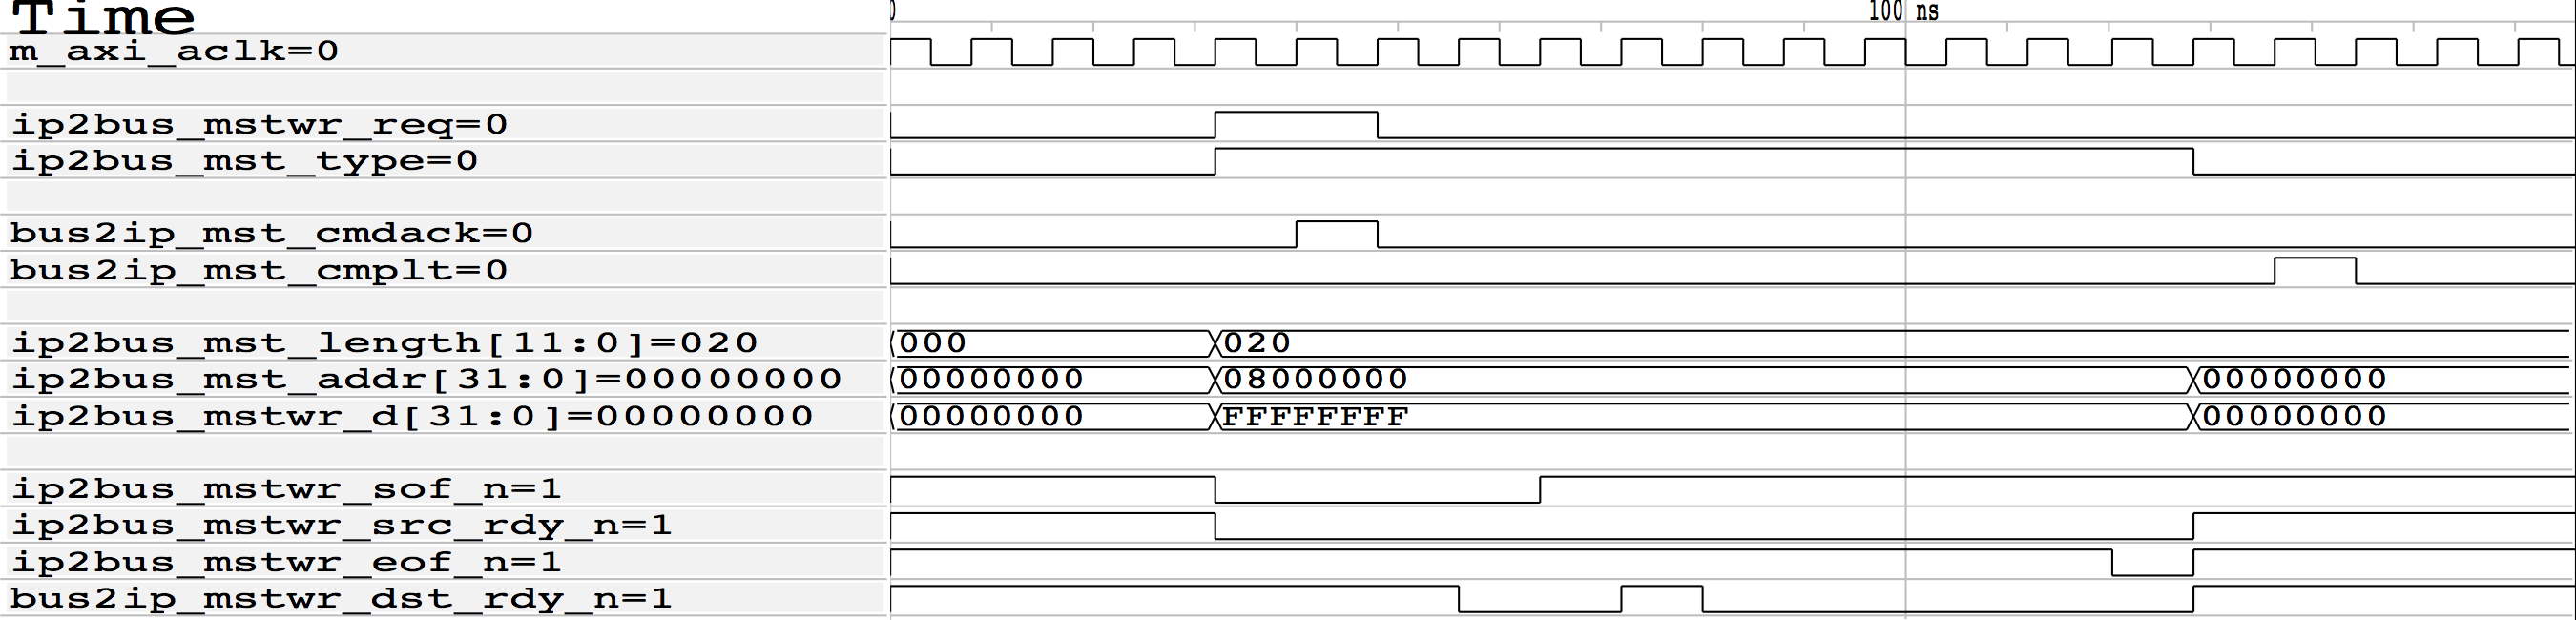
\includegraphics[width=\textwidth] {images/communication/ambwriteburst.png}
    \caption{\texttt{axi\_master\_burst} burst write transaction}
    \label{fig:ambwrburst}
\end{figure}

To test the UDP File Transfer stack in the simulator, a model of the 
\texttt{axi\_master\_burst} is defined in \texttt{axi\_master\_burst\_model}.
The model behaves on the IP side like the real IP core but does not need an AXI
slave that receives or sends data. 
\\

The memory address is calculated in equation \ref{eq:rxadrcalc}. This calculation implies
a multiplication of the packet data size times the data sequence number. To
minimize logic utilization \texttt{c\_pkg\_uft\_rx\_pack\_size} is set to
\texttt{1024} so this operation is simply a shift operation. However this leads
to a loss in data throughput. 
\begin{equation}
    axi\_adr = c\_pkg\_uft\_rx\_base\_addr + c\_pkg\_uft\_rx\_pack\_size * data\_seq
    \label{eq:rxadrcalc}
\end{equation}

% ==============================================================================
%
%                             Transmitter
%
% ==============================================================================
\clearpage
\subsection{Transmitter}
The transmitter is split into two paths. The command assembler and the data
assembler. The two blocks are controlled by the \texttt{uft\_tx\_ctrl} entity.
The \texttt{uft\_tx\_cmd\_assembler} reads the inputs shown in table 
\ref{tab:ufttxsig} and creates a AXI data stream according to the UFT command
packet specification. After the packet is sent the control block then starts the
\texttt{uft\_tx\_data\_assembler}. It reads the data to be sent into a 32 in, 8
out FiFo block (the inverse to that described in chapter \ref{chapt:uftreceiver}) and
instantaneously begins transmission. The two AXI stream sources need to be
connected to a single AXI stream sink (the UDP IP stack). This is done by the
\texttt{uft\_tx\_arbiter}. It switches between the command assembler and data
assembler according to the signal coming from the control block.
\\

The \texttt{uft\_tx\_ctl} block takes the data base address and the number of
bytes to be sent and then controls the command and data packet generation. The
file transfer start packet (see \ref{tab:uftcommandlist}) requires the number of
sequences that will be sent. Therefore the \texttt{uft\_tx\_ctl} has to
calculate this number using the \texttt{data\_size} and UFT packet
specification. This ceiling division is done in listing \ref{lst:nseq}.
\\

\begin{table}[h!]
    \centering
    \begin{tabular}{l l}
        \toprule
        Signal & Description \\
        \midrule
        \texttt{uft\_tx\_ctl} & {} \\
        \midrule
        \texttt{data\_size} & Number of bytes to send\\
        \texttt{data\_src\_addr} & Data source base address \\
        \texttt{tx\_ready} & Indicates if the system is ready for a new file transfer \\
        \texttt{tx\_start} & Assert high to start a transmission \\

        \midrule
        \texttt{uft\_tx\_cmd\_assembler} & {} \\
        \midrule
        \texttt{en\_start} & Start command packet generation\\
        \texttt{done} & Asserted high if command is sent\\
        \texttt{data\_size} & Number of sequences to send (NSEQ)\\
        \texttt{tcid} & Transaction ID\\

        \midrule
        \texttt{uft\_tx\_data\_assembler} & {} \\
        \midrule
        \texttt{start} & Start data packet generation\\
        \texttt{done} & Asserted high if data is sent\\
        \texttt{data\_src\_addr} & Data address on AXI Bus\\
        \texttt{tcid} & Transaction ID \\
        \texttt{seq} & Packet sequence number\\
        \texttt{size} & Number of bytes to send\\
        \bottomrule
    \end{tabular}
    \caption{UFT Tx block interface signals}
    \label{tab:ufttxsig}
\end{table}

\clearpage
\begin{minipage}{\linewidth}
    \begin{lstlisting}[
        style=VHDLStyle, 
        caption=NSEQ calculation, 
        label=lst:nseq
        ]
    cmd_nseq <= (data_size / c_nbytes_per_packet)
                when data_size(1 downto 0) = "00" else
                (data_size / c_nbytes_per_packet) + 1);\end{lstlisting}
\end{minipage}

% ==============================================================================
%
%                             Implemented Features
%
% ==============================================================================
\subsection{Implemented Features}
The UDP File transfer is a proof of concept. Its protocol specification is
preliminary and not yet fully implemented neither on a computer nor on the
FPGA. This chapter lists the implemented features.
\\

The \textbf{receiver} is capable of receiving data packets of any length and
number of sequences. The data packets also do not have to arrive in order.
If the packet payload size is not a power of two, a
multiplier is synthesized that requires more area than a simple shift if a power
of two (maximum 1024) is used. Unimplemented features are:
\begin{itemize}
    \item Data packet acknowledgment (command ACKFP), therefore an error free
    file reception is not guaranteed
    \item File transfer acknowledgment (command ACKFT)
    \item Transaction ID (TCID) check
    \item UDP checksum validation is not supported by the UDP IP Stack
\end{itemize}

The \textbf{transmitter} can send files of any size in a four byte step, this is
due to the fact that an AXI read is four bytes. The file transfer start (FTS)
command is sent with the correct values. The NSEQ calculation requires a
divider if a packet size anything else than a power of two is used.
Unimplemented features are:
\begin{itemize}
    \item Data packet acknowledgment (command ACKFP) check
    \item File transfer acknowledgment (command ACKFT) check
    \item Data retransmission if acknowledge failed
    \item UDP header checksum generation
\end{itemize}
Currently a data transfer with multiple data packets (NSEQ > 1) is slowed down
by a 100$\mu s$ delay between packets to prevent a buffer overflow on the
receiving
computer.




